\section{Tracking multiobjeto}
\label{sec:tracking-tecnologias}

El tracking multiobjeto consiste en mantener la identidad de múltiples objetos a lo largo de una secuencia de vídeo. A diferencia de la detección de objetos, que produce resultados independientes en cada frame, el tracking introduce una asociación temporal entre detecciones consecutivas. Su objetivo es asignar un identificador persistente a cada objeto, de forma que pueda reconstruirse su trayectoria a lo largo del tiempo.

Este problema suele abordarse combinando detección, predicción de movimiento y asociación de detecciones. En cada frame, el detector proporciona un conjunto de cajas candidatas. A continuación, el tracker compara estas detecciones con las trayectorias activas y decide qué detección corresponde a cada identidad previa, qué objetos han desaparecido temporalmente y qué detecciones deben iniciar nuevas trayectorias. Esta asociación puede basarse en medidas geométricas, como el solape entre cajas, la distancia entre posiciones o la coherencia del movimiento estimado.

\subsection{ByteTrack}
ByteTrack \citep{ZhangByteTrack2022} es una de las referencias recientes más relevantes en tracking multiobjeto. Su principal aportación consiste en no descartar directamente las detecciones con baja confianza, ya que algunas de ellas pueden corresponder a objetos reales parcialmente ocluidos, lejanos o difíciles de detectar. En lugar de ello, ByteTrack utiliza estas detecciones en una segunda etapa de asociación, lo que permite recuperar trayectorias que otros métodos podrían fragmentar.

El funcionamiento de ByteTrack puede entenderse como un ciclo que se repite en cada frame. En primer lugar, el detector proporciona un conjunto de cajas con sus puntuaciones de confianza. Estas detecciones se separan en dos grupos mediante umbrales: detecciones de alta confianza, que se consideran más fiables, y detecciones de baja confianza, que no son suficientes para iniciar nuevas trayectorias pero sí pueden servir para actualizar trayectorias ya existentes.

Antes de realizar la asociación, las trayectorias activas se predicen hacia el frame actual mediante un filtro de Kalman \citep{Kalman1960}. Este filtro estima la posición esperada de cada objeto a partir de su estado anterior, habitualmente representado mediante la posición y tamaño de la caja. De esta forma, el tracker no compara las nuevas detecciones con la última posición observada sin más, sino con una predicción de dónde debería encontrarse cada objeto en el frame actual.

La asociación se realiza en varias fases. En la primera fase, ByteTrack compara las trayectorias activas y perdidas recientemente con las detecciones de alta confianza. Para ello calcula una matriz de costes basada normalmente en la IoU entre cajas, de modo que una detección se asocia a una trayectoria si su solape con la predicción del track es suficientemente alto. Las asociaciones válidas actualizan el estado del track y mantienen su identidad.

Después, las trayectorias que no han podido asociarse en la primera fase se comparan con las detecciones de baja confianza. Esta segunda asociación es la característica distintiva de ByteTrack. Una detección de baja confianza no se utiliza para crear un nuevo objeto, ya que podría ser ruido o fondo, pero sí puede ser útil para mantener una trayectoria ya existente cuando el detector ha reducido temporalmente su seguridad. De este modo, un jugador parcialmente oculto o detectado con baja confianza puede seguir asociado a su identidad previa.

Además de los tracks activos, ByteTrack mantiene otros estados internos. Los tracks no confirmados corresponden normalmente a trayectorias recién creadas que todavía no han sido observadas durante suficientes frames (si no se asocian de nuevo rápidamente, se eliminan). Los tracks perdidos son identidades que no han encontrado una detección compatible en el frame actual, pero que se conservan durante un número limitado de frames por si el objeto reaparece. Si un track permanece perdido durante más tiempo del permitido por el parámetro de memoria del tracker, se marca como eliminado. Finalmente, las detecciones de alta confianza que no han sido asociadas a ningún track existente pueden iniciar nuevas trayectorias si superan un umbral mínimo de confianza.

La \hyperref[fig:bytetrack-esquema]{Figura~\ref*{fig:bytetrack-esquema}} resume este proceso. Primero se realiza la asociación con detecciones de alta confianza. Después, las trayectorias no asociadas se comparan con detecciones de baja confianza. Luego, las trayectorias no confirmadas se comparan con detecciones de alta confianza. Por último, se actualizan los estados de las trayectorias, se crean nuevos tracks cuando procede y se eliminan aquellos que han permanecido perdidos durante demasiado tiempo.

\begin{figure}[H]
    \centering
    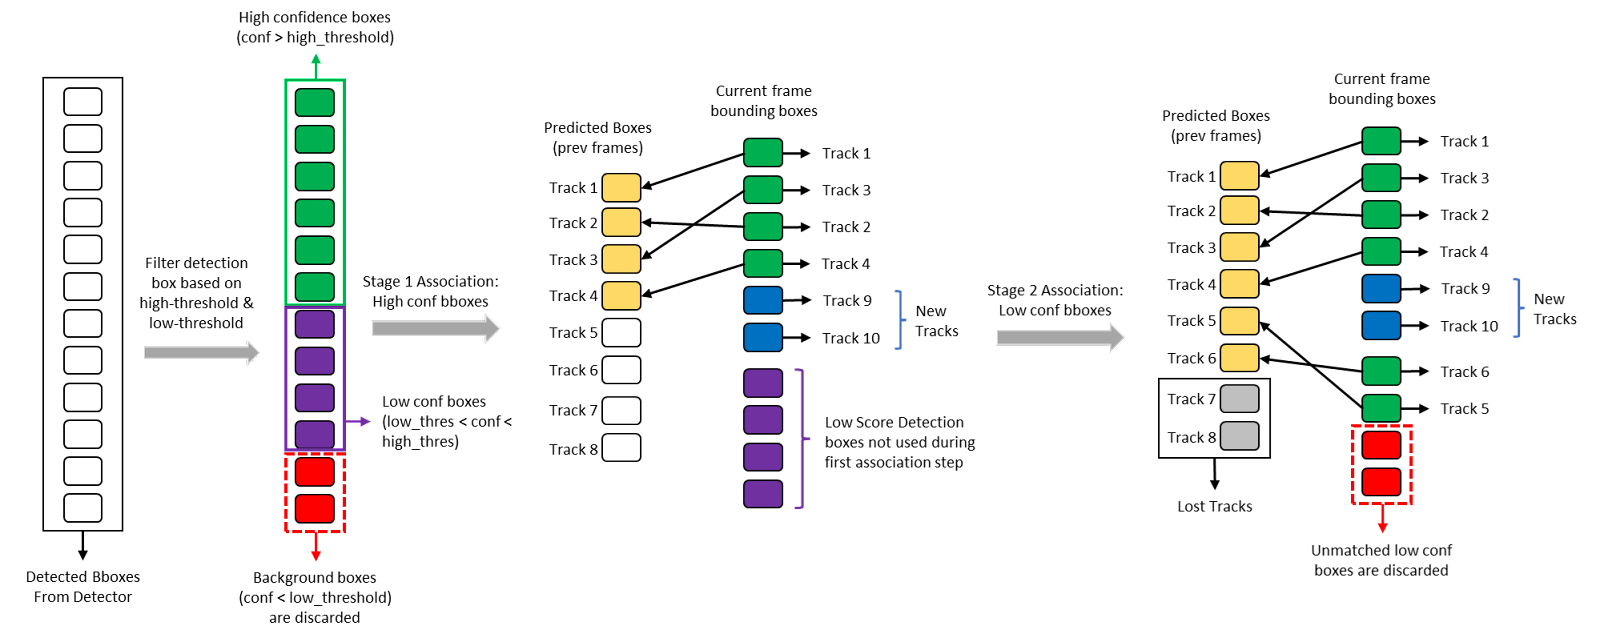
\includegraphics[width=0.9\textwidth]{Imagenes/Propias/ByteTrack.png}
    \caption[Esquema general de ByteTrack]{Esquema general de ByteTrack. El método separa las detecciones en cajas de alta y baja confianza y realiza la asociación en dos etapas, permitiendo recuperar objetos que un tracker convencional descartaría prematuramente. Fuente: reproducido de So \citep{SoByteTrack2025}.}
    \label{fig:bytetrack-esquema}
\end{figure}

Esta estrategia resulta especialmente útil en secuencias con oclusiones, movimiento rápido, cambios de escala o detecciones intermitentes. Además, ByteTrack mantiene una arquitectura relativamente simple y eficiente, ya que basa la asociación principalmente en predicción de movimiento, solape espacial y confianza de detección, sin depender necesariamente de descriptores complejos de apariencia. Esto facilita su integración en sistemas donde la latencia y la estabilidad temporal son factores importantes.

\subsection{Papel del tracking dentro del pipeline}

En este proyecto, el tracking multiobjeto permite transformar las detecciones independientes de cada frame en trayectorias persistentes de jugadores, árbitros, porteros y balón. Esta continuidad temporal es necesaria para analizar la evolución del juego y para que módulos posteriores, como la clasificación posicional o la detección de eventos puedan trabajar sobre identidades estables y analizar su evolución temporal.

El vídeo broadcast de fútbol plantea dificultades específicas para esta tarea: oclusiones frecuentes, cruces entre jugadores, similitud visual entre miembros del mismo equipo, cambios de escala, movimientos de cámara y detecciones intermitentes. Por ello, ByteTrack se utiliza como base del sistema, pero se adapta al dominio futbolístico incorporando señales adicionales y restricciones sobre las asociaciones posibles.

En nuestro caso, ByteTrack se utiliza como punto de partida, pero se realiza una profunda adaptación a nuestro caso de uso. El objetivo es aprovechar la estructura eficiente de ByteTrack, incorporando al mismo tiempo información específica del fútbol. Por tanto, el criterio de asociación no se basa únicamente en la IoU entre cajas, sino que también considera la clase detectada, el equipo estimado, la distancia entre centros de las cajas y, cuando está disponible, la posición proyectada sobre el terreno de juego. Además, se introducen restricciones duras para evitar asociaciones incompatibles y fases adicionales de asociación para recuperar correspondencias cuando el solape entre cajas no resulta suficiente.

Estas adaptaciones buscan reducir cambios de identidad, trayectorias fragmentadas y asociaciones incoherentes, problemas especialmente relevantes en un entorno como el fútbol. La implementación concreta de la capa de asociación basada en ByteTrack dentro del pipeline se describe posteriormente en la \hyperref[sec:bytetrack-layer]{Sección~\ref*{sec:bytetrack-layer}}.